%% Sample file $Id: PBML_article.tex 134 2010-07-01 19:28:04Z popel $
\documentclass{pbml}
%\documentclass[nofonts]{pbml} % for XeLaTeX without Pagella and DejaVu fonts

\usepackage{color,fancyvrb}
\definecolor{gray}{rgb}{0.9,0.9,0.9}
\usepackage{amsmath}
%\renewcommand*\ttdefault{txtt} % 20% tighter than courier

% This is a sample file for the PBML article.
% You can compile it with (ordered by preference)
%  1. XeLaTeX with installed fonts TeX Gyre Pagella and DejaVu
%  2. XeLaTeX without the fonts -> you must use \documentclass[nofonts]{pbml}
%  3. pdfLaTeX
%
% In all three methods, you can use Unicode (utf8) encoding for special letters
% (so instead of na\"{i}ve you can write directly naïve).
% Note that with methods 2 and 3, your output will be slightly DIFFERENT than
% our final print version (different line breaks and page breaks).
% See the end of this file for more information.

% Packages
% ========
% In this place you can load required packages by the \usepackage commands.
% The following packages are loaded automatically by the class:
% euler    (for math fonts)
% graphicx (for inclusion of images)
% multicol (for multicolumn typesetting)
% natbib   (for bibliography citations)
% amssymb  (for various symbols)
% If XeLaTeX is used, fontspec and xltxtra are loaded as well.

% Definitions
% ===========
% You can use your own macros defined by \newcommand, \providecommand,
% \DeclareRobustCommand (or even by \def) as well as environments declared by
% \newenvironment. These definitions will automatically be local to your
% article and will not clash with other parts of the journal. You can also
% use \newcounter in order to declare your own counters.

% This switches to color version and is explained below (sec. Color Images).
% \graphicspath{{./color/}{./grayscale/}}    

\begin{document}


% Document title and authors
% ==========================
% Due to journal organization, the article title and authors must be specified
% AFTER \begin{document}. Note that \subtitle is not allowed anymore due to
% problems with indexing in science databases. If needed use colon in the title.

\title{An Experimental Management System}


% Now put the affiliated institutes first, then author names and the labels
% of their institutes in the "institute" field. The order of institutes and
% authors printed below the title will be the same as the order of your commands.
% Each author can be associated with more than one institute.
% One author must be chosen as the "corresponding author" (using attribute
% corresponding) and his or her email and full address must be provided.
% PLEASE, use Unicode (utf8) encoding (e.g ï instead of \"{i}).

\institute{label1}{University of Edinburgh}

\author{
  firstname=Philipp,
  surname=Koehn,
  institute=label1,
  corresponding=yes,
  email={pkoehn@inf.ed.ac.uk},
  address={School of Informatics\\ University of Edinburgh\\ Scotland, United Kingdom}
}

% If all authors belong to the same institute, you can use simpler syntax:
% \institute{}{Institute of Formal and Applied Linguistics, Charles University in Prague}
% \author{firstname=Humpty, surname=Dumpty}
% \author{firstname=Mock, surname=Turtle,
%   corresponding=yes,
%   email={turtle@seacoast.wl},
%   address={Institute of Formal and Applied Linguistics\\
%            Charles University in Prague\\
%            Malostranské náměstí 25\\
%            118 00 Praha 1, Czech Republic}}
% \author{firstname=Cheshire, surname=Cat}


% The title and authors' names are used in the running head. If they are
% long, you should define short versions. These definitions are optional. You
% define them only if they are needed. The example follows:
\shorttitle{Experimental Management System}
\shortauthor{P. Koehn}

% Now print the title by:
\maketitle


% Abstract
% ========
% The abstract is placed within the "abstract" environment. It is a mandatory
% part of the article.

\begin{abstract}
We describe Experiment.perl, an experimental management system, that allows the execution of the entire training and testing pipeline of a machine translation experiment with one configuration files. When carrying out multiple experimental runs with changed settings, Experiment.perl automatically detects which steps need to be re-run and which can be re-used.
\end{abstract}


% In addition to the \cite command, you can use natbib style of citations:
%\citet{PDT2} shows \ldots \\
%\ldots tree-based annotation (as e.g.~\citealp{PDT2}).

% For figures and tables always use "figure" resp. "table" floating environments
% and always supply a caption. See the paragraph about color images below.




\section{\label{experiment-perl.texntoc1}Introduction}

Running a machine translation experiment involves many steps: preparing training data, building language and translation models, tuning, testing, scoring and analysis of the results. For most of these steps, a different tool needs to be invoked, so this easily becomes very cumbersome.
The Experiment Management System (EMS), or Experiment.perl, for lack of a better name, makes it much easier to run experiments. It ships with the Moses machine translation toolkit \citep{koehn-EtAl:2007:PosterDemo}.

\begin{figure}
\begin{center}
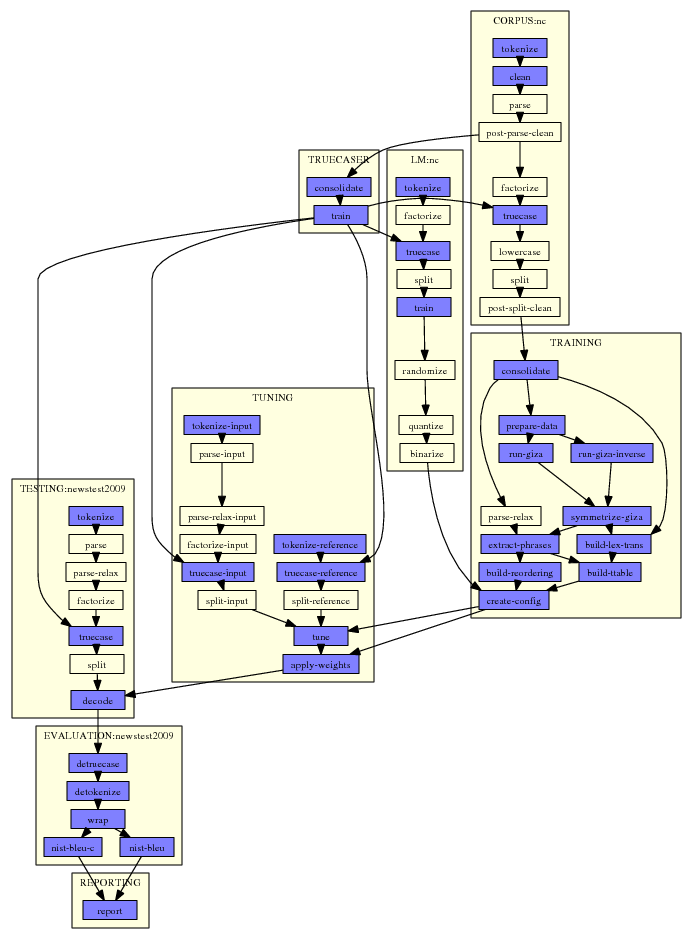
\includegraphics[scale=0.45]{ems-agenda.png}
\end{center}
\caption{{\bf Workflow generated by Experiment.perl:} Steps (such as {\tt run-giza} are grouped into modules (such as {\tt TRAINING}). Dependencies are indicated by arrows. Skipped steps have a pale background.}
\label{ems-agenda}
\end{figure}

A typical example is given in Figure~\ref{ems-agenda}.
The graph was automatically generated by Experiment.perl. All that needed to be done was to specify one single configuration file that points to data files and settings for the experiment.
In the graph, each step is a small box. For each step, Experiment.perl builds a script file that gets either submitted to a compute cluster or executed on the same machine. Note that some steps are quite involved, for instance tuning: On a cluster, the tuning script runs on the head node a submits jobs to the queue itself.



Experiment.perl makes it easy for multiple experimental runs with different settings]. It automatically detects which steps do not have to be executed again.
Experiment.perl plays the same role as LoonyBin \citep{loonybin}, but there are significant differences in its usage. Experiment.perl uses a textual configuration file to set up an experiment and a meta configuration file to define all possible workflows, LoonyBin offers a graphical user interface that lets the user connect steps.




\section{Design}

Experiment.perl breaks up training, tuning, and evaluating of a statistical machine translation system into a number of steps, which are then scheduled to run in parallel or sequence depending on their inter-dependencies and available resources. The possible steps are defined in the file {\tt experiment.meta}. An experiment is defined by a configuration file.

\subsection{Experiment.Meta}


The actual steps, their dependencies and other salient information is to be found in the file {\tt experiment.meta}. Think of {\tt experiment.meta} as a "template" file.
Steps are grouped into modules, which are:

\begin{itemize}
\item {\tt CORPUS}: preparing a parallel corpus

\item {\tt INPUT-FACTOR} and {\tt OUTPUT-FACTOR}: commands to create factors

\item {\tt TRAINING}: training a translation model

\item {\tt LM}: training a language model

\item {\tt INTERPOLATED-LM}: interpolate language models

\item {\tt SPLITTER}: training a word splitting model

\item {\tt RECASING}: training a recaser

\item {\tt TRUECASING}: training a truecaser

\item {\tt TUNING}: running minumum error rate training to set component weights

\item {\tt TESTING}: translating and scoring a test set

\item {\tt REPORTING}: compile all scores in one file

\end{itemize}

To give an example of a step definition in {\tt experiment.meta}, here the parts of the definition for {\tt LM:get-corpus} and {\tt LM:tokenize}:

\vspace{2mm}
\begin{SaveVerbatim}{myverb}
 get-corpus
        in: get-corpus-script
        out: raw-corpus
        [...]

 tokenize
        in: raw-corpus
        out: tokenized-corpus
        [...]
\end{SaveVerbatim}
\colorbox{gray}{%
\BUseVerbatim{myverb}
}
\vspace{2mm}

Each step takes some input ({\tt in}) and provides some output ({\tt out}). This also establishes the dependencies between the steps. The step {\tt tokenize} requires the input {\tt raw-corpus}. This is provided by the step {\tt get-corpus}.

The file {\tt experiment.meta} provides a generic template for steps and their interaction. For an actual experiment, a configuration file determines which steps need to be run. This configuration file is specified when invoking {\tt experiment.perl}. It may contain for instance the following:

\vspace{2mm}
\begin{SaveVerbatim}{myverb}
 [LM:europarl]

 ### raw corpus file
 #
 raw-corpus = $europarl-v3/training/europarl-v3.en
\end{SaveVerbatim}
\colorbox{gray}{%
\BUseVerbatim{myverb}
}
\vspace{2mm}

Here, the corpus to be used for language modeling is named {\tt europarl} and it is provided in raw text format in the location {\tt \$europarl-v3/training/europarl-v3.en} (the variable {\tt \$europarl-v3} is defined elsewhere in the config file). The effect of this specification in the config file is that the step {\tt get-corpus} does not need to be run, since its output is given as a file. The workflow starts with the step {\tt tokenize}.

The entire definition of an experiment follows this logic, which is very similar to the principles of a Unix Makefile. The ultimate purpose of an experiment is to generate a result file at the end. If this is not given, then scoring scripts need to be called. Scoring scripts require the output of the decoder on the test sets. The decoder requires a tuned model. Tuning requires a trained model. Trained models require language models and model files, and so on. The workflow, as show in Figure~\ref{ems-agenda}, is generate bottom up, following the input/output dependencies of steps.

\subsection{Elements of Step Definitions}

Several parameters for step definitions are used in {\tt experiment.meta}:

\begin{itemize}
\item {\tt in} and {\tt out}: Established dependencies between steps; input may also be provided by files specified in the configuration.

\item {\tt default-name}: Name of the file in which the output of the step will be stored.

\item {\tt template}: Template for the command that is placed in the execution script for the step.

\item {\tt template-if}: Potential command for the execution script. Only used, if a specified setting exists.

\item {\tt error}: Experiment.perl detects if a step failed by scanning {\tt STDERR} for key words such as killed, error, died, not found, and so on. Additional key words and phrase are provided with this parameter.

\item {\tt not-error}: Declares default error key words as not indicating failures.

\item {\tt pass-unless}: Only if the given setting is used, this step is executed, otherwise the step is passed (illustrated by a yellow box in the graph).

\item {\tt ignore-unless}: If the given setting is used, this step is not executed. This overrides requirements of downstream steps.

\item {\tt rerun-on-change}: If similar experiment are runs, the output of steps may be used, if input and settings are the same. This specifies settings whose change disallows a re-use in different run.

\item {\tt parallelizable}: When running on a cluster or a multi-core machine, this step may be parallelized (only if {\tt generic-parallelizer} is set in the config file).

\item {\tt qsub-script}: If running on a cluster, this step is run on the head node, and not submitted to the queue (because it submits jobs itself).

\end{itemize}

To complete our example, the full definition of the step {\tt LM:tokenize} is below.

\vspace{2mm}
\begin{SaveVerbatim}{myverb}
 tokenize
         in: raw-corpus
         out: tokenized-corpus
         default-name: lm/tok
         pass-unless: output-tokenizer
         template: $output-tokenizer < IN > OUT
         parallelizable: yes
\end{SaveVerbatim}
\colorbox{gray}{%
\BUseVerbatim{myverb}
}
\vspace{2mm}

The step takes {\tt raw-corpus} and produces {\tt tokenized-corpus}. It is parallizable with the generic parallelizer. 
The output is stored in the file according to the definition {\tt corpus/tok}. Note that the actual file name also contains the corpus name, and the run number. In our example the tokenized corpus is stored in a file named  {\tt lm/europarl.tok.1}. 
The step is only executed, if {\tt output-tokenizer} is specified. The template indicate how the command lines in the execution script for the steps are formed.

\subsection{Multiple Corpora, One Translation Model}

We may use multiple parallel corpora for training a translation model or multiple monolingual corpora for training a language model (or use multiple language models). Each of these have their own instances of the {\tt CORPUS} and {\tt LM} module. There may be also multiple test sets in {\tt TESTING}). However, there is only one translation model and hence only one instance of the {\tt TRAINING} module. 
The definitions in {\tt experiment.meta} reflects the different nature of these modules. For instance {\tt CORPUS} is flagged as {\tt multiple}, while {\tt TRAINING} is flagged as {\tt single}.

When defining settings for the different modules, the singular module {\tt TRAIN\-ING} has only one section, while this one general section and specific {\tt LM} sections for each training corpus. In the specific section, the corpus is named, e.g. {\tt LM:europarl}.
When looking up the parameter settings for a step, first the set-specific section ({\tt LM:europarl}) is consulted. If there is no definition, then the module definition ({\tt LM}) and finally the general definition (in section {\tt GENERAL}) is consulted. In other words, local settings override global settings.

\subsection{Configuration File}

A configuration file for an experimental run consists of a collection of settings, one per line with empty lines and comment lines for better readability, organized in sections for each of the modules.

The start of each section is indicated by the section name in square brackets ({\tt [TRAINING]} or {\tt [CORPUS:europarl]}). If the word {\tt IGNORE} is appended to a section definition, then the entire section is ignored.

The syntax of setting definition is {\tt setting = value} (note: spaces around the equal sign). If the value contains spaces, it must be placed into quotes ({\tt setting = "the value"}), except when a vector of values is implied (only used when defining list of factors: {\tt output-factor = word pos}. 
Comments are indicated by a hash ({\tt \#}). 

Settings can be used as variables to define other settings:

\vspace{2mm}
\begin{SaveVerbatim}{myverb}
 working-dir = /home/pkoehn/experiment
 wmt10-data = $working-dir/data
\end{SaveVerbatim}
\colorbox{gray}{%
\BUseVerbatim{myverb}
}
\vspace{2mm}

Variable names may be placed in curly brackets for clearer separation:

\vspace{2mm}
\begin{SaveVerbatim}{myverb}
 wmt10-data = ${working-dir}/data
\end{SaveVerbatim}
\colorbox{gray}{%
\BUseVerbatim{myverb}
}
\vspace{2mm}

Such variable references may also reach other modules:

\vspace{2mm}
\begin{SaveVerbatim}{myverb}
 [RECASING]
 tokenized = $LM:europarl:tokenized-corpus
\end{SaveVerbatim}
\colorbox{gray}{%
\BUseVerbatim{myverb}
}
\vspace{2mm}

Finally, reference can be made to settings that are not defined in the configuration file, but are the product of the defined sequence of steps. 
Say, in the above example, {\tt tokenized-corpus} is not defined in the section {\tt LM:europarl}, but instead {\tt raw-corpus}. Then, the tokenized corpus is produced by the normal processing pipeline. Such an intermediate file can be used elsewhere:

\vspace{2mm}
\begin{SaveVerbatim}{myverb}
 [RECASING]
 tokenized = [LM:europarl:tokenized-corpus]
\end{SaveVerbatim}
\colorbox{gray}{%
\BUseVerbatim{myverb}
}
\vspace{2mm}

Some error checking is done on the validity of the values in the configuration file before an experimental run is executed. All values that seem to be file paths trigger the existence check for such files. A file with the prefix of the value must exist.

\subsection{Step Files}
Let us follow our example of the tokenization step in the language model module in more detail. Recall that the {\tt LM:europarl} section has a specification of {\tt raw-corpus} to {\tt \$europarl-v3/train\-ing/europarl-v3.en}. Since only the raw corpus, but not a tokenized corpus is specified, Experiment.perl concludes that it needs to run the tokenization step.

The directory {\tt steps} contains the script that executes each step, its {\sc stderr} and {\sc stdout} output, and meta information:

\vspace{2mm}
\begin{SaveVerbatim}{myverb}
 steps/1/LM_europarl_tokenize.1
 steps/1/LM_europarl_tokenize.1.DONE
 steps/1/LM_europarl_tokenize.1.INFO
 steps/1/LM_europarl_tokenize.1.STDERR 
 steps/1/LM_europarl_tokenize.1.STDERR.digest
 steps/1/LM_europarl_tokenize.1.STDOUT
\end{SaveVerbatim}
\colorbox{gray}{%
\BUseVerbatim{myverb}
}
\vspace{2mm}

The file {\tt steps/1/LM\_europarl\_tokenize.1} is the shell script that is run to execute the step. The file with the extension {\tt DONE} is created when the step is finished - this communicates to the scheduler that subsequent steps can be executed. The file with the extension {\tt INFO} contains meta information - essential the settings and dependencies of the step. This file is checked to detect if a step can be re-used in subsequent experimental runs.

In case that the step crashed, we expect some indication of a fault in {\tt STDERR} (for instance the words {\tt core dumped} or {\tt killed}). This file is checked to see if the step was executed successfully, so subsequent steps can be scheduled or the step can be re-used in new experiments. Since the {\tt STDERR} file may be very large (some steps create Megabytes of such output), a digested version is created in {\tt STDERR.digest}. If the step was successful, it is empty. Otherwise it contains the error pattern that triggered the failure detection.

\subsection{Re-Use of Steps}

Let us now take a closer look at re-use. If we run the experiment again but change a settings, say, the order of the language model, then there is no need to re-run the tokenization, but only language model training.

Here is the definition of the language model training step in {\tt experiment.meta}:

\vspace{2mm}
\begin{SaveVerbatim}{myverb}
 train
   in: split-corpus
   out: lm
   default-name: lm/lm
   ignore-if: rlm-training
   rerun-on-change: lm-training order settings
   template: $lm-training -order $order $settings -text IN -lm OUT
   error: cannot execute binary file
\end{SaveVerbatim}
\colorbox{gray}{%
\BUseVerbatim{myverb}
}
\vspace{2mm}

The mention of {\tt order} in the list behind {\tt rerun-on-change} informs experiment.perl that this step does need to be re-run, if the order of the language model changes. Since none of the settings in the chain of steps leading up to the training have been changed, those can be re-used.

If the language model order is changed and the experiment.perl is run again in the same working directory, you will see the following files in the directory {\tt lm}:

\vspace{2mm}
\begin{SaveVerbatim}{myverb}
 % ls -tr lm/*
 lm/europarl.tok.1
 lm/europarl.truecased.1
 lm/europarl.lm.1
 lm/europarl.lm.2
\end{SaveVerbatim}
\colorbox{gray}{%
\BUseVerbatim{myverb}
}
\vspace{2mm}

Note that a new language model was trained for this second run ({\tt lm/europarl.lm.2}), but no new tokenized and truecased corpus files. These were re-used from run 1.

Steps are re-used from previous runs, unless settings listed under {\tt rerun-on\--change} are changed, one of its specified input files (if any) are changed, and if one of its previous steps are re-run. Note that if a filename is not changed, but its time stamp differs, this triggers re-running a step. This ensures that only a minimum number of steps are run to produce the exact same outcome as if all steps are run.

\subsection{Web Interface and Analysis}

Experiment.perl also offers a web interface to the experimental runs for easy access and comparison of experimental results. The web interface gives a listing of experiments and runs for each experiments, with a display of automatic metric scores, and links to configuration files and outputs.

You can include additional analysis for an experimental run in the web interface by specifying the setting {\tt analysis} in its configuration file.
This adds reports n-gram precision and recall statistics and color-coded n-gram correctness markup for the output sentences to the web interface. See Figure~\ref{ems-annotation} for an example. 

\begin{figure}
\begin{center}
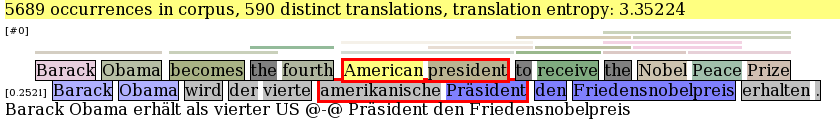
\includegraphics[scale=0.45]{ems-annotation.png}
\end{center}
\caption{Comparing outputs from two experimental runs}
\label{ems-annotation}
\end{figure}

The output is color-highlighted according to n-gram matches with the reference translation. The following colors are used. The darker the color of an output word, the higher n-gram match to the reference translation it is part of.

Additional reports are available when adding the  settings {\tt analyze-coverage} and {\tt report-segmentation}.
The setting {\tt analyze-coverage} include a coverage analysis: which words and phrases in the input occur in the training data or the translation table? This is reported in color coding and in a yellow report box when moving the mouse of the word or the phrase. Also, summary statistics for how many words occur how often are given, and a report on unknown or rare words is generated.


The setting {\tt report-segmentation} creates summary statistics about what kind of phrase mappings are used (one word to one word, 1-2, 2-2, etc.), as well as markup of the sentence pair with the phrase segmentation. The phrase segmentation is indicated with black boxes around the words, and the alignment is shown when moving the mouse on the phrases.

\section{Usage}

\subsection{Quick Start}

Experiment.perl is extremely simple to use:

\begin{itemize}
\item Find {\tt experiment.perl} in {\tt scripts/ems}

\item Get a sample configuration file from someplace (for instance {\tt scripts/ems/exam\-ple/config.toy}).

\item Set up a working directory for your experiments for this task ({\tt mkdir} does it).

\item Edit the following path settings in {\tt config.toy}
\begin{itemize}
\item {\tt working-dir}

\item {\tt data-dir}

\item {\tt moses-script-dir}

\item {\tt moses-src-dir}

\item {\tt srilm-dir}

\item {\tt decoder}

\end{itemize}

\item Run {\tt experiment.perl -config config.toy} from your working directory.

\item Marvel at the graphical plan of action.

\item Run {\tt experiment.perl -config config.toy -exec}.

\item Check the results of your experiment (in {\tt evaluation/report.1})

\end{itemize}


\subsection{More Examples}


The {\tt example} directory contains some additional examples. 
These require the training and tuning data released for the Shared Translation Task for WMT 2010.

The examples using these corpora are

\begin{itemize}
\item a basic phrase based model

\item a factored phrase based model

\item a hierarchical phrase based model

\item a target syntax model

\end{itemize}


The factored model using all the available corpora is identical to the Edinburgh submission \citep{koehn-EtAl:2010:WMT} to the WMT 2010 shared task for English-Spanish, Spanish-English, and English-German language pairs. The French language pairs also used the $\text{10}^\text{9}$ corpus, the Czech language pairs did not use the POS language model, and German-English used additional pre-processing steps.

\section{Outlook}
We have been using Experiment.perl for years and are satisfied with its core functionalities. In future work, we would like support job scheduling on Hadoop clusters and extend the analysis facility.

\section*{Acknowledgments}
This work was supported in part by the EuroMatrixPlus project funded by the 
 European Commission (7th Framework Programme) and in part under the GALE program of the 
 Defense Advanced Research Projects Agency, Contract No. HR0011-06-C-0022.

\bibliography{more,mt,WMT-2010}

\end{document}

